\section{Density matrix and entropy for network}
%as in paper 2023 with the special case in paper 2020
The communicability matrix defined above possesses peculiar properties that make it suitable for use as a density matrix. Moreover, the presence of the Laplacian matrix ensures that it does not only consider the topological features of the network but also the dynamics. Taking the exponential communicability matrix as a reference, we can define a density matrix as
\begin{equation}\label{density_matrix}
    \hat \rho(\beta) = \frac{1}{Z} e^{-\beta \hat L} \qquad \mathrm{with} \qquad Z(\beta) = \Tr[e^{-\beta \hat L}],
\end{equation}
where $Z$ is the partition function and it is equal to the Laplacian Estrada index of the network \eqref{EE_L}.
It is a Hermitian and positive defined matrix with trace equal to unity. 
It can be seen that $e^{-\beta L}$ is the propagator of the master equation \eqref{random_walk_solution} in a network at time $t = \beta$.

From this, we can define the network's entropy as the Von Neumann entropy
\begin{equation} \label{entropy}
    S(\hat\rho) = -\Tr[\hat \rho \ln \hat \rho].
\end{equation}
The entropy is not negative and it is equal to zero if and only if the $\hat\rho$ is a pure state. It has a higher bound $S \leq \ln(N)$,  \cite{Nielsen_Chuang_2010}.
The entropy satisfy the sub-additivity property \cite{De_Domenico_2016}:
Let $\hat\rho$, $\hat\tau$ and $\hat\sigma$ be density matrices corresponding to the networks $G$, $H$, $I$ respectively. The networks $t$ and $S$ are subgraph of the network $G$ such that $G = H + I$.
If the sub-additivity is satisfied  then $S(\hat\rho) \leq S(\hat\tau) + S(\hat\sigma)$, the equivalence is obtain if the two subgraphs does not have nodes from the same component of $G$. In appendix \ref{C_sub_additivity} there is a mathematical proof.
Figure \ref{fig:ER-BA-WS} shows the entropy \eqref{entropy} for different types of networks\footnote{The python scripts can be found in the GitHub page of the author at the link: \url{https://github.com/ShqemzaMatteo/Master_thesis}}: a ring graph, an Erd\H{o}s-Rényi (E-R) random graph, a Barab\'asi-Albert (B-A) scale-free graph, and a Watts-Strogatz (W-S) small-sworld graph.

\begin{figure}[ht!]
    \centering
    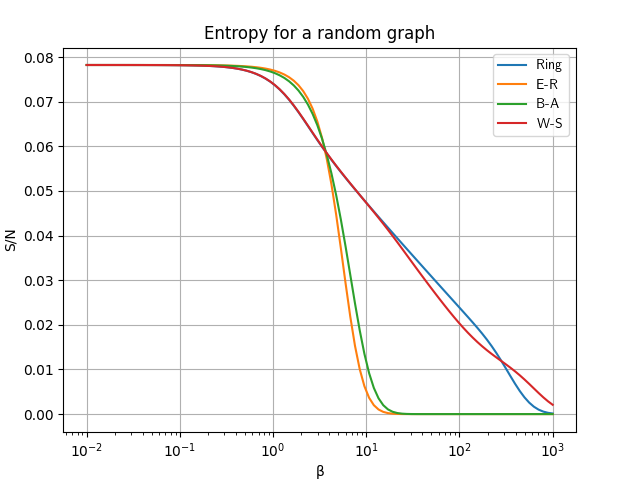
\includegraphics[width=0.80\linewidth]{image/random_graph.png}
    \caption{Plot of the network's entropy per node as a function of $\beta$ for different network types with $50$ nodes: a ring graph (blue), a Erd\H{o}s-Rényi (E-R) random graph with connectivity probability $0.7$ (orange), a Barab\'asi-Albert (B-A) scale-free graph with parameter $m=3$ (green), and a Watts-Strogatz (W-S) small world graph with parameter $K=3$ and rewire probability 0.2 (red). The x-axis has a logarithmic scale. For large $\beta$ the entropy tends to zero far all the networks.}
    \label{fig:ER-BA-WS}
\end{figure}

%Using the density matrix, we can introduce also other thermodynamics quantities like the Helmoltz free energy $F = -\frac{1}{\beta} \ln Z$.


A possible interpretation of this density matrix is given by De Domenico \cite{De_Domenico_2020}.
Consider a network $G(N,M)$, represented by the adjacency matrix $A$. In this network a classic particle walks. 
The network can be described using the Dirac notation. Let be $\ket{\psi} = \sum_i \rho_i \ket{i}$ the state of the system, where $\ket{i}$ is the canonical vector identifying the node $i$ and $\rho_i$ is the probability to find the particle on top of node $i$. Thus, the scalar product $\braket{i}{\psi} = \rho_i$ is already an observable. The set $\{\ket{i}\}_{i=0}^N$ forms an orthogonal basis, satisfying $\braket{i}{j} = \delta_{ij}$, where $\delta_{ij}$ is the Kronecker delta. 
The evolution of the dynamics is governed by the Laplacian operator $\hat L = L_{ij} \ket{i}\bra{j}$ following the equation
\begin{equation} \label{time_evolution}
    \partial_t \ket{\psi(t)} = - \hat L \ket{\psi(t)},
\end{equation}
with the solution
\begin{equation}
    \ket{\psi(t)} = \hat G(t,0) \ket{\psi(0)}
\end{equation}
where $\hat G(t,0) = e^{-t\hat L}$ is the propagator and $\ket{\psi(0)}$ is the initial state. 

If the detailed balance condition \eqref{detail_condition} holds, $\hat L$ is Hermitian. Therefore, the propagator can be diagonalized in the orthogonal basis $\{\ket{v_\lambda}\}_\lambda$ of eigenvectors of the control operator as
\begin{equation}\label{diagonal_propagator}
    \hat G(t,0) = \sum_\lambda e^{-t\lambda} \ket{v_\lambda}\bra{v_\lambda} = \sum_\lambda e^{-t\lambda} \hat \sigma_\lambda,
\end{equation}
where $\hat \sigma_\lambda = \ket{v_\lambda}\bra{v_\lambda}$ is the projector over the left and right eigenvectors with the $\lambda$ eigenvalue. The operators do not depend on time, they are constant along the process, only the coefficients change.
The system relaxes to a stationary state $\ket{\psi_0}$ corresponding to the zero eigenvector.

We consider the system in the initial state $\ket{\psi} = \ket{\psi_0} + \ket{\Delta\psi}$, where $\ket{\Delta\psi}$ is a small perturbation relative to the stationary state. The initial perturbation can be decomposed between the different nodes as $\ket{\Delta\psi_0} = \sum_i \Delta_i \ket{i}$.
The time evolution of the initial state becomes
\begin{equation}
    \ket{\psi(t)} = G(t,0) \ket{\psi(0)} = \ket{\psi_0} + G(t,0)\ket{\Delta\psi} = \ket{\psi_0} + \ket{\Delta\psi(t)}
\end{equation}
with $\ket{\Delta\psi(t)} = e^{-t\hat L} \ket{\Delta \psi}$.

Since the stationary component is constant in time, we focus on the evolution of the perturbation $\ket{\Delta\psi_0}$. 
The value of the perturbation on top of node $j$ at time $t$ is
\begin{equation}
    \braket{j}{\Delta\psi(t)} = \bra{j} e^{-t\hat L} \ket{\Delta\psi} =\sum_\lambda \bra{j} e^{-t\lambda} \hat \sigma_\lambda\ket{\Delta\psi} = \sum_i  \sum_\lambda \Delta_i e^{-t\lambda} \bra{j}  \hat \sigma_\lambda \ket{i}.
\end{equation}
We have used equation \eqref{diagonal_propagator} and the definition of the perturbation.
This equation shows that the perturbation can travel through $N$ different streams, one for each projector $\sigma_\lambda$, with the stream's size $\Delta_i e^{-t\lambda}$. If $\Delta_i e^{-t\lambda} > 0$ the stream is active; if $\Delta_i e^{-t\lambda} = 0$ it is inactive. Negative stream coefficients imply an inverted flux from $j$ to $i$.
Now, we assume that there is maximal uncertainty on the perturbation, therefore $\Delta_i = \Delta$.
The dynamics can traps part of the perturbation in a specific node. The trapped perturbation's size can be compute as
\begin{equation}\label{T_equation}
    T = \sum_i  \sum_\lambda \Delta e^{-t\lambda} \bra{i}  \hat \sigma_\lambda \ket{i} = \Delta \Tr [\hat G(t,0)]
\end{equation} 
The density matrix is defined as
\begin{equation}
    \hat\rho(t) = \frac{1}{Z}\sum_\lambda  e^{-t\lambda} \hat \sigma_\lambda = \frac{1}{Z} e^{-t\hat L},
\end{equation}
where $Z = \Tr[e^{-t\hat L}] $ is the partition function.
The evolution of the perturbation can be written as
\begin{equation}
    \braket{j}{\Delta\psi(t)} = \sum_i \Delta Z \bra{j}\hat\rho(t) \ket{i}.
\end{equation}
The stream's size are proportional to the trapped field.
This density matrix can be interpreted as the probability that the perturbation will flow through a specific stream $\hat \sigma_l$ at time $t$ in the ensemble of all the possible streams \cite{De_Domenico_2020}. We have recovered the density matrix \eqref{density_matrix} considering the time $t$ as the parameter $\beta$.

The complexity of information streams can be quantified by the Von Neumann entropy.
When the information dynamics is described by a single information stream, entropy vanishes: the density matrix is a pure state.
In contrast, as the information dynamics becomes more complex and diverse, the number of information streams increases resulting in higher entropy: the density matrix is a mixed state.

Considering the analogy with the quantum mechanics, in the following chapters we propose another way to obtain the density matrix \eqref{density_matrix} starting from the quantum walk instead of the classic one. The new description, based on open quantum system, has add new meaning to the network's entropy \eqref{entropy}.

\subsection{Kullback-Leibler and Jensen-Shannon Divergences}
Starting from the concept of entropy, we can also introduce the Kullback-Leibler (KL) divergence or relative entropy \cite{K-L_divergence} as
\begin{equation}\label{KL_divergence}
    D_{KL}(\hat \rho || \hat \sigma) = \Tr \left[\hat \rho \ln\left(\frac{\hat\sigma}{\hat\rho}\right)\right].
\end{equation}
It measure the how much close is the distribution $\hat \sigma$ to reproduce a event with real distribution $\hat \rho$. 
The KL divergence is always non negative and it equals zero when $\hat \rho = \hat \sigma$. It is not symmetric and unbounded \cite{J-S_divergence}.

It can be used to make comparisons between networks. Moreover, this concept can be applied to the reconstruction of network starting from real data using the maximum likelihood estimation: it consist in finding the best model that reproduces the experimental data minimizing the Kullback-Leibler divergence between a chosen network model and the dataset \cite{De_Domenico_2016}. This opens the door to the application of machine learning technique in network theory.

However the Kullback-Leibler divergence is not symmetric, therefore it can not be use as a metric. 
But we can symmetrize introducing the Jensen-Shannon (JS) divergence \cite{J-S_divergence} defined as
\begin{equation}\label{JS_metric}
    \mathcal{D}_{JS}(\hat\rho||\hat\sigma) =  \frac{1}{2}D_{KL}(\hat \rho || \hat \mu) + \frac{1}{2}D_{KL}(\hat \sigma || \hat \mu) = S(\hat\mu)-\frac{1}{2}\left[S(\hat\rho) + S(\hat\sigma)\right],
\end{equation}
where $\hat\mu =\frac{1}{2}(\hat\rho+\hat\sigma)$. 

The JS divergence is a bounded function \cite{J-S_divergence}
\begin{equation}
    0 \geq \mathcal{D}_{JS}(\hat\rho||\hat\sigma) \geq 1.
\end{equation}
$\left(\mathcal{D}_{JS}\right)^{\frac{1}{2}}$ defines a metric: it is symmetric, positive define, and hold the triangular inequality \cite{Jensen-Shannon_divergence}. 
%It has been use successfully to measure the distance between the layer of a multilayer network in order to aggregate them and eliminate the redundant layers \cite{multilayer}.

Figure \ref{Fig:JS_divergence} shows the Jensen-Shannon divergence between an Erd\H{o}s-Rényi (E-R) random graph, a Barab\'asi-Albert (B-A) scale-free graph and a Watts-Strogatz (W-S) small-sworld graph \footnote{The python scripts can be found in the GitHub page of the author at the link: \url{https://github.com/ShqemzaMatteo/Master_thesis}}.

\begin{figure}[ht!]
    \centering
    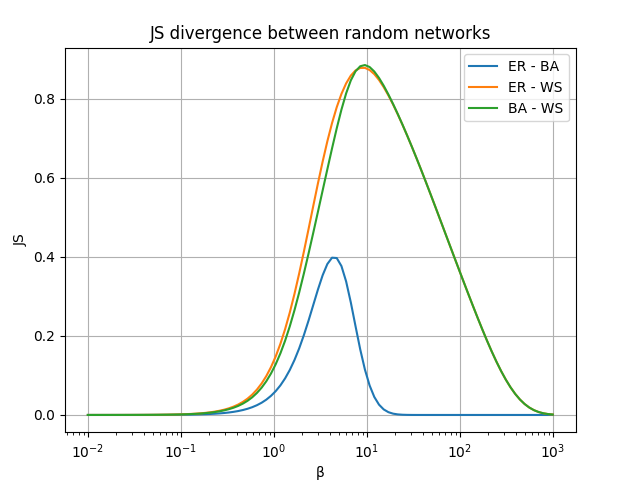
\includegraphics[width=0.80\textwidth]{image/JS_divergence.png}
    \caption{Plot of the KL divergence as a function of $\beta$ between different network types with $50$ nodes: a Erd\H{o}s-Rényi (E-R) random graph with connectivity probability $0.7$ and a Barab\'asi-Albert (B-A) scale-free graph with parameter $m=3$ (blue); a Erd\H{o}s-Rényi (E-R) random graph with connectivity probability $0.7$ and Watts-Strogatz (W-S) small world graph with parameter $K=3$ and rewire probability 0.2 (orange); a Barab\'asi-Albert (B-A) scale-free graph with parameter $m=3$ and a Watts-Strogatz (W-S) small world graph with parameter $K=3$ and rewire probability 0.2 (green). The x-axis has a logarithmic scale.The ER and BA networks are closer respect to a WS network. The divergence is maximum around $\beta = 10$.}
    \label{Fig:JS_divergence}
\end{figure}
It has been use successfully to measure the distance between the layer of a multiplex network.
In some system the elements can interacts with different type of interaction, to models them we create a set of networks with same number of node but different links, one for each interaction's type. Each network form a layer for a multiplex. For example, the mobility inside a city can be mapped into a multiplex, one layer for each means of transport. Multiplex with many layers are difficult to handle, in order to simplify the model we use the JS divergence to aggregate the redundant layer \cite{multilayer}.

However, both the KL and JS divergences study only the spectrum properties of the system. Thus, they do not distinguish between different networks with same spectrum but different eigenvector.